\chapter{Fundamentação teórica}

\section{PISCINAS e sua manutenção}

    \subsection{HISTÓRICO E POPULARIZAÇÃO DAS PISCINAS}

        \textcolor{red}{Foi pedido a redução desse tópico, concentrando-se na difusão residencial a partir do século XX.}
    
        Piscina que vem do latim piscis “peixe”, pode ser definida como um tanque cheio de água com inúmeros fins, sejam eles: Natação, mergulhos, saltos ornamentais ou simplesmente para fins recreativos\cite{piscinaOquee}. Com registros desde 2600 A.C "Os Grandes Banhos de Mohenjodaro" considerado um dos primeiros tanques de água pública, feito de tijolos e coberto por gesso. Contudo, acredita-se que esse tanque foi feito apenas para fins religiosos.
         \begin{figure}[H]
         	\centering
         	\caption{ }  
        	\centering
         	\label{fig:cont}
        	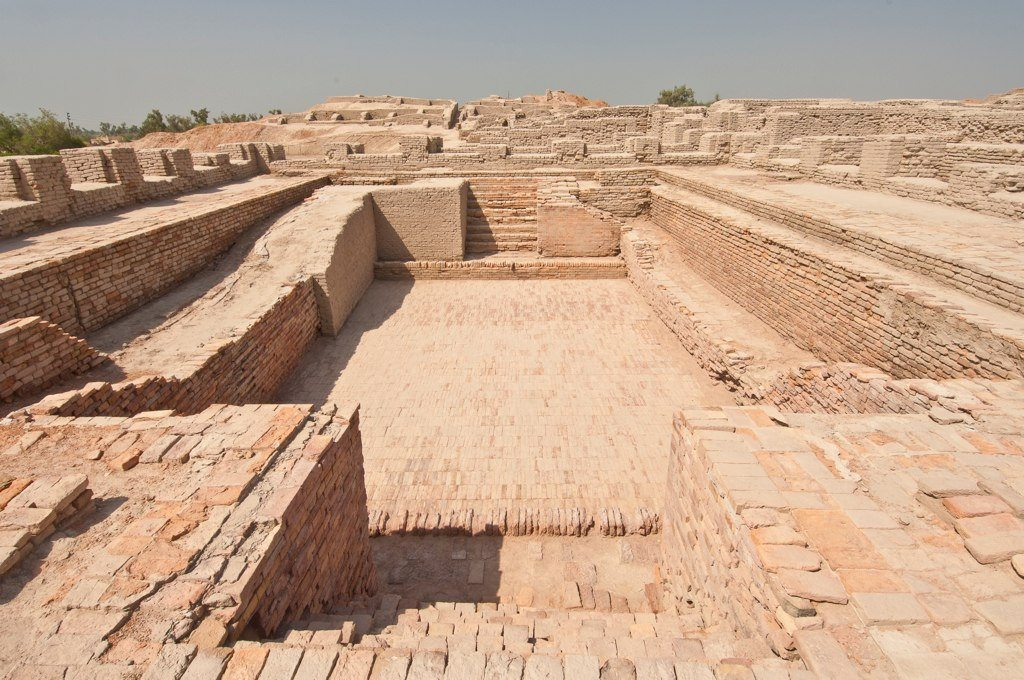
\includegraphics[width=0.78\textwidth]{imagens/primeiraPiscina.png}
        	\caption*{Fonte: Fibratec}
         \end{figure}

         \textcolor{green}{Removi o paragrafo que fala sobre a Grécia antiga deixando a parte sobre o século XX e deixei o primeiro.}
        
        Com o avanço da tecnologia no século 20, as piscinas foram recebendo novos sistemas, como a cloração e filtração que disponibilizavam água limpa para a piscina que anteriormente era necessário ter a troca completa da água para ser limpa. No ocidente as piscinas começaram a se popularizar com a invenção do gunite (mistura de cimento, areia e água), um material que facilitava a instalação, possibilitava projetos mais flexíveis e um custo bem mais baixo\cite{piscinaHistoria}.

        \textcolor{red}{Colocar mais sobre o presente como ela se popularizou de fato}

    \subsection{COMPONENTES BÁSICOS DE UMA PISCINA}
        \textcolor{red}{Colocar os componentes básicos de uma piscina e explica-los de forma rápida}
    
        \textcolor{blue}{Segundo \cite{refComponents} as piscinas de forma abstrata, são extremamente simples, sendo apenas grandes reservatórios de água para o uso recreativo. Podendo existir diferentes tipos como: piscina de ondas do parque aquático, particular, pública e entre outras. Contudo, em sua maioria todas as piscinas possuem alguns componentes básicos que são necessários para a filtração e tratamento químico.}

        \textcolor{blue}{Diante disso, se deve ter uma mínima noção dos componentes que a mesma possui, sendo eles: bomba motorizada, filtro de água, alimentador químico, drenos, devoluções e encanamentos de PVC e em alguns casos pode haver um aquecedor a fim de manter a temperatura da piscina mais elevada.}

        \begin{itemize}
        
            \item \textcolor{blue}{Bomba Motorizada:}
                \textcolor{blue}{Responsável por circular toda a água, puxando da bacia e levando até outros processos.}

            \item \textcolor{blue}{Filtro de Água:}
                \textcolor{blue}{Remover parte das impurezas da água como: folhas, poeiras e micro-organismos.}

            \item \textcolor{blue}{Alimentador Químico:}
                \textcolor{blue}{Distribuir os produtos químicos responsáveis pela limpeza da piscina.}

            \item \textcolor{blue}{Drenos:}
                \textcolor{blue}{Removem a água utilizada para limpeza, escoamento ou manutenção.}

            \item \textcolor{blue}{Devoluções:}
                \textcolor{blue}{Pontos de reabastecimento da água da piscina.}

            \item \textcolor{blue}{Encanamentos de PVC:}
                \textcolor{blue}{Liga todos os componentes da piscina, permitindo todo o transporte da água.}
                %Colocar uma imagem de cada item respectivo ou uma no final que tenha todos
                
        \end{itemize}

        \begin{figure}[H]
         	\centering
         	\caption{ }  
        	\centering
         	\label{fig:cont}
        	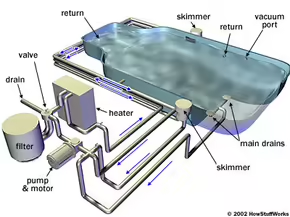
\includegraphics[width=0.48\textwidth]{imagens/componentesPiscina.png}
            \caption*{Componentes básicos de uma piscina}
        	\caption*{Fonte: \cite{refComponents}}
         \end{figure}

        \textcolor{blue}{Todos esses componentes tem como objetivo bombear a água em um ciclo contínuo, passando por todos os sistemas, como filtragem, e tratamento químico, porém, ainda existem os componeres que são responsáveis por auxiliar na limpeza física.}

         \textcolor{red}{colocar os componentes para a limpeza física}
        

    \subsection{NORMAS E PROCEDIMENTOS TÉCNICOS DE LIMPEZA MANUAL}

       \textcolor{red}{Desenvolver com base nas normas da ABNT (como NBR 10339 - Instalação de piscinas) e manuais técnicos. Explicar a frequência de limpeza, produtos obrigatórios, riscos do uso incorreto, etc.}

       \textcolor{blue}{Segundo a \cite{piscineiroProfissional}, a falta de um procedimento correto de limpeza de uma piscina, pode vir a acarretar sérios problemas de saúde para aquelas que a utilizam, como: Dermatite, micose e outros. Seu tratamento deve ser constante e feito de forma eficiente, tal qual o resultado seja sempre o determinado segundo normas regidas pela ABNT. De acordo com \cite{guiaTratamento} são diversos os fatores poluentes de uma piscina, porém, é de extrema importância citar alguns deles como: Suor e urina; pelos e cabelos; óleos de pele; insetos; folhas; formação de algas; e diversos outros.}

       \textcolor{blue}{Tais poluentes podem afetar diretamente os parâmetros químicos de uma piscina, como o pH e o cloro. Segundo \cite{guiaTratamento}, efetuando uma limpeza física utilizando escovas ou redes, só é possível remover a parte visível dos poluentes, como: Folhas, insetos e lodo. Por isso surge também a necessidade de efetuar um tratamento químico efetivo, pois outros tipos de poluentes como o suor ou urina, se misturam com a água. Tal acontecimento se deve pelos agentes filtrantes serem incapazes de filtrar certos poluentes.}

       %Tentar inserir alguma imagem no final de algum desses três paragrafos pois esta tudo muito grande

       \textcolor{blue}{É de suma importância que uma piscina limpa atenda a alguns pré-requisitos, que são eles: Ausência de bactérias do grupo coliforme ou Staphylococcus aureus\footnote{Bactéria que fica alojada no nariz} , uma boa visibilidade do fundo da piscina, superfície livre de sujeiras e o pH na faixa ideal entre 7,2 e 7,8. Diante disso, para se obter esses pré-requisitos exigidos, é importante que a água possua esses três princípios básicos:}
    
       \begin{itemize}
            \item \textbf{\textcolor{blue}{Água Limpa:}} \textcolor{blue}{Água transparente e sem a presença de sedimentos.}
            
            \item \textbf{\textcolor{blue}{Água Balanceada:}} \textcolor{blue}{Segundo todos os parâmetros prescritos, sem risco de prejudicar o banhista.}
             
            \item \textbf{\textcolor{blue}{Água Saudável:}} \textcolor{blue}{Livre de micro-organismos que podem vir a prejudicar o banhista.}
            
        \end{itemize}

        \begin{figure}[H]
                \centering
                \caption{ }  
            	\centering
                \label{fig:cont}
            	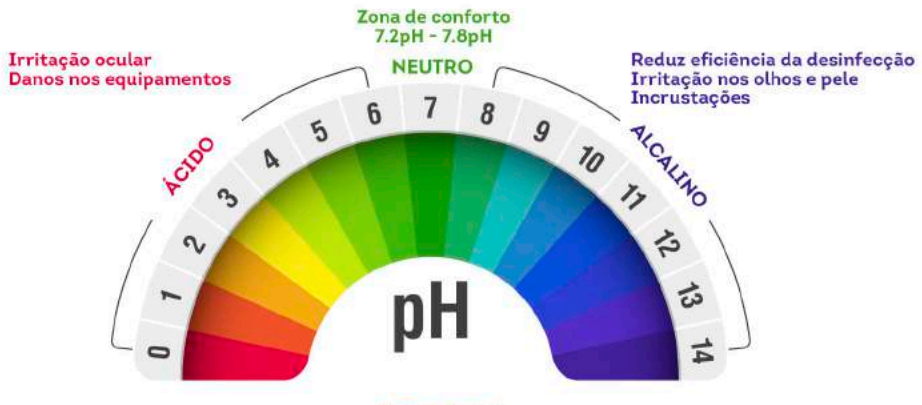
\includegraphics[width=0.48\textwidth]{imagens/medidorPh.png}
                \caption*{Faixa de pH}
            	\caption*{Fonte: \cite{guiaTratamento}}
        \end{figure}


        \textcolor{blue}{Antes da limpeza é importante ter o conhecimento da área e o volume da piscina, para que seja utilizado a quantidade correta de produtos para obter uma limpeza precisa e livre de desperdícios. Para calcular a área e o volume pode ser utilizado diferentes formulas dependendo do formato da piscinas, segue as formulas:}

        \subsubsection*{\textcolor{blue}{Piscina Retangular}}
        
            \[
            A = \text{comprimento} \times \text{largura}
            \]
            \[
            V = \text{comprimento} \times \text{largura} \times \text{profundidade}
            \]
            
        \subsubsection*{\textcolor{blue}{Piscina Circular}}
            \[
            A = \pi r^2
            \]
            \[
            V = \pi r^2 h
            \]
            
        \subsubsection*{\textcolor{blue}{Piscina Oval (Elíptica)}}
            \[
            A = \pi \cdot \frac{a}{2} \cdot \frac{b}{2}
            \]
            \[
            V = A \cdot h
            \]
            
            \textcolor{blue}{Nos casos em que a piscina possui fundo inclinado, a profundidade considerada deve ser a média entre a parte mais rasa e a mais funda:}
            \[
            h_m = \frac{h_{\text{maior}} + h_{\text{menor}}}{2}
            \]
            

        \textcolor{blue}{Segundo \cite{tccSilva} o processo de limpeza é similar ao utilizado em industrias como em uma Estação de tratamento de água, seguindo uma sequência de cinco etapas.}

        \begin{itemize}
            \item \textbf{\textcolor{blue}{Oxidação:}} \textcolor{blue}{Ocorre a mistura do cloro a fim de oxidar metais como ferro e manganês para facilitar a retirada de matéria orgânica}
            
            \item \textbf{\textcolor{blue}{Coagulação e Floculação:}} \textcolor{blue}{Consiste na junção de sulfato de alumínio e, esporadicamente, cloreto férrico para desequilibrar as partículas, seguindo pela circulação da água para formar flocos}
             
            \item \textbf{\textcolor{blue}{Decantação:}} \textcolor{blue}{Acontece quando as particulas coaguladas e floculadas se alojam no fundo da piscina, em razão da circulação lenta do fluido. Dependendo do produto utilizada, essa etapa pode durar cerca de 6 horas.}

            \item \textbf{\textcolor{blue}{Filtração:}} \textcolor{blue}{Contenção do acumulo de sujeira das etapas anteriores, que geralmente é feito por um filtro de areia.}

            \item \textbf{\textcolor{blue}{Correção de pH:}} \textcolor{blue}{Análise e ajuste do pH da água, geralmente utilizando um medidor para identificar o valor. O procedimento evita a deterioração dos canos.}
            
        \end{itemize}

        \textcolor{blue}{Em virtude do exposto, torna-se evidente que aplicar de forma correta os procedimentos técnicos estabelecidos é indispensável para uma melhor manutenção da qualidade da água. Neste sentido, a precisão e a segurança demandadas pelo processo dependem diretamente da escolha e do manuseio adequado dos produtos químicos, tema que será abordado na próxima seção.}


    \subsection{PRODUTOS QUÍMICOS E ACESSÓRIOS USADOS NA LIMPEZA DE PISCINAS}
        \textcolor{red}{Manter. Expandir explicando pH ideal, uso de cloro, algicidas, floculantes, entre outros}

        \textcolor{blue}{O tratamento preciso e bem executamo na hora da limpeza de uma piscina, tanto o físico como químico, garantem uma boa qualidade da água, a fim de evitar possíveis infecções ou doenças transmitidas pela água. Por isso, é importante entender quais produtos utilizar e como utilizar, bem como entender a melhor forma de efetuar o tratamento físico. O principal objetivo dessa seção é mostrar quais produtos e ferramentas se deve utilizar para garantir uma boa qualidade da água e evitar possíveis doenças para o usuário.}

        \begin{itemize}
        
            \item \textbf{\textcolor{blue}{Precedimento Químico:}} \textcolor{blue}{Segundo \cite{guiaTratamento}, é todo a parte que envolve a adição de produtos químicos na água para garantir sua qualidade e evitar riscos a saúde dos usuários, ajustando a alcalinidade o pH e também garantindo a desinfecção da água pelos micro-organismos e bactérias utilizando cloro, bem como outros produtos com o intuído de tratar outros parâmetros. Abaixo está uma tabela com os produtos e a quantidade adequada que deve ser colocada a cada mil litros.}

                \begin{figure}[H]
                    \centering
                    \caption{ }  
                	\centering
                    \label{fig:cont}
                	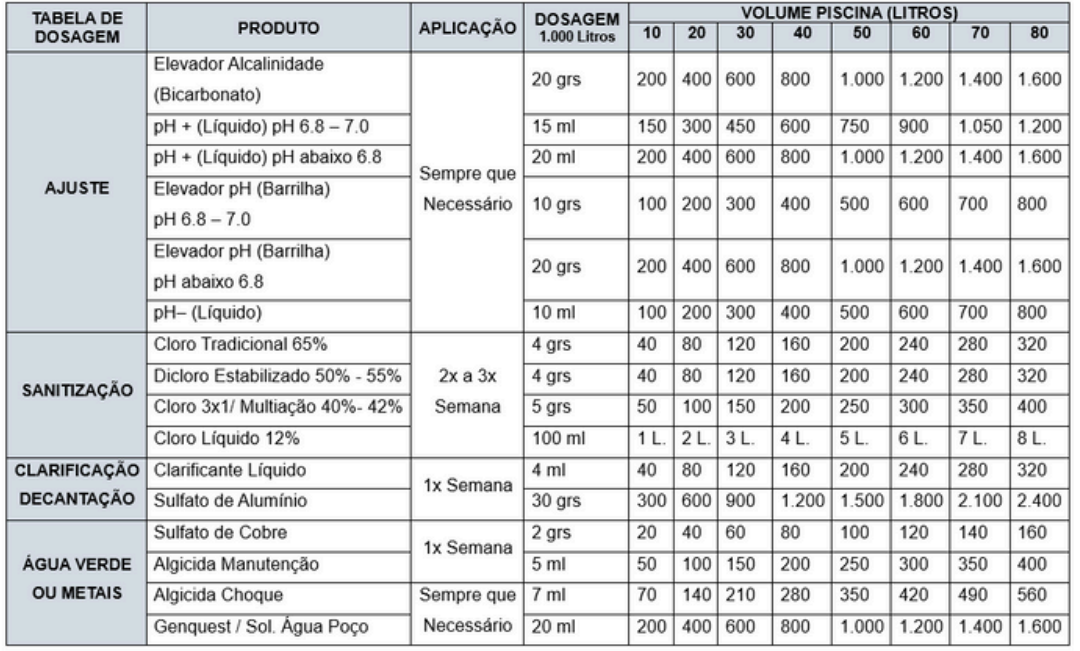
\includegraphics[width=1.00\textwidth]{imagens/tabelaProdutos.png}
                    \caption*{Tabela de Dosagem de Produtos}
                	\caption*{Fonte: \cite{guiaTratamento}}
                \end{figure}
    
                \begin{itemize}
    
                    \item \textbf{\textcolor{blue}{Elevador de Alcalinidade:}} \textcolor{blue}{A alcalinidade da água está relacionado com a sua capacidade de neutralizar ácidos, se comportando como uma especie de contenção para manter o pH estável. O elevador de alcalinidade tem como objetivo elevar a alcalinidade para o nível ideal que é entre 80 a 120 ppm.}
    
                    \item \textbf{\textcolor{blue}{Barrilha, Elevador de pH, pH+:}} \textcolor{blue}{Produtos com sua composição alcalina que tem como principal função elevar o pH quando baixo.}
    
                    \item \textbf{\textcolor{blue}{Redutor de pH, pH-:}} \textcolor{blue}{Composição ácida que tem a função de diminuir o pH}
    
                    \item \textbf{\textcolor{blue}{Hipoclorito de Sódio, Cloro, Dicloro, Multiação 3x1:}} \textcolor{blue}{Produtos Sanetizantes que basicamente tem como objetivo eliminar os micro-organismos na água.}
    
                    \item \textbf{\textcolor{blue}{Sulfato de Alumínio, Clarificantes:}} \textcolor{blue}{Faz as partículas de sujeira presente na piscina passem por um processo chamado decantação que em resumo, aglomera as partículas e as leva para o fundo da piscina, facilitando o processo de aspiração e filtração.}
    
                    \item \textbf{\textcolor{blue}{Sulfato de Cobre, Algicida:}} \textcolor{blue}{É utilizando quando a piscina chega no processo de esverdeada, eliminando algas e o lodo.}
    
                    \item \textbf{\textcolor{blue}{Genquest, Solução Água de poço:}} \textcolor{blue}{Remove manchas e cores de metais dissolvidos na água da piscina.}
    
                \end{itemize}
                
            \item \textbf{\textcolor{blue}{Medição de Parâmetros e Ajuste do pH:}} \textcolor{blue}{Para medir os parâmetros deve-se utilizar estojos de analise do respectivo parâmetro que vai ser analisado. Ajustar os parâmetros são o ponto chave para um tratamento eficiente da água. Segue um exemplo de estojo para a analise de diferentes parâmetros como o pH, cloro e Alcalinidade.}

            \begin{figure}[H]
                    \centering
                    \caption{ }  
                	\centering
                    \label{fig:cont}
                	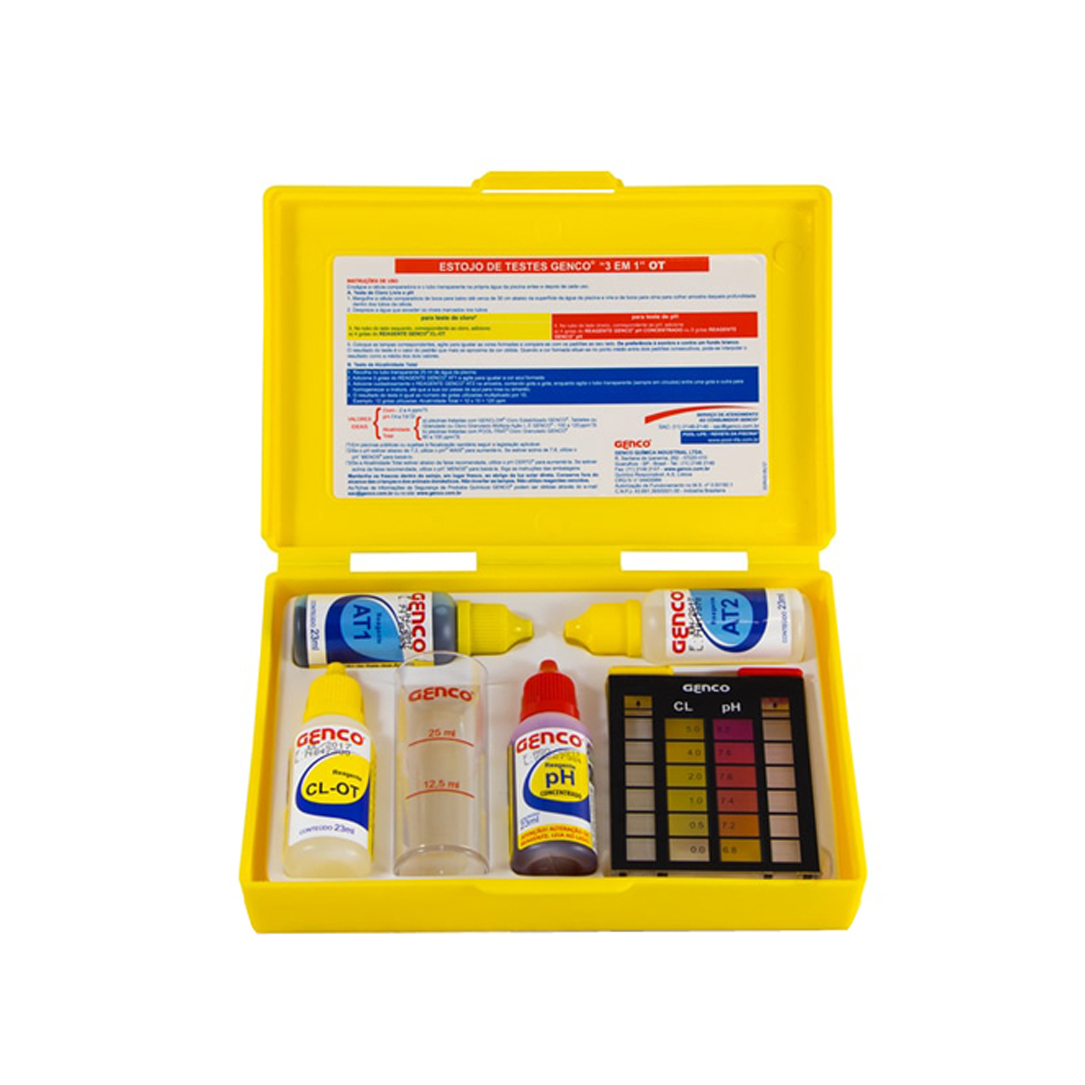
\includegraphics[width=0.48\textwidth]{imagens/estojoMedidor.png}
                    \caption*{Estojo para Análise de Parâmetros}
                	\caption*{Fonte: \cite{gencoEmpresa}}
            \end{figure}

            %Colocar imagens de medidor
            \textcolor{blue}{Os produtos a serem utilizados dependem da alteração e do parâmetro alterado, caso o pH apareça abaixo de 7, se deve usar o elevador de pH ou o barrilha, se a Alcalinidade constar abaixo do ideal, é necessário utilizar o elevador de Alcalinidade, e por fim, se o cloro estiver baixo também, será necessário aplicar cloro liquido ou granulado, como consta na tabela mostrada anteriormente.}


            \item \textbf{\textcolor{blue}{Limpeza Fisica:}} \textcolor{blue}{Dado as informações fornecidadas até o presente momento, deve-se ter um entendimento sobre a turbidez da água, que é a presença de particulas em suspensão na água. Para fazer o devido tratamento, é recomendado fazer o uso fazer o uso de um decantador que aglomera as particulas de sujeira levando-as para o fundo da piscina para que possa ser feita a devida aspiração. Dito isso, existes algumas maneiras de resolver esse problema, são elas: Clarificação que deve ser feito quando a água estiver opaca e sem brilho e a Floculaçao ou decantação, que deve ser utilizando quando a água estiver turva ou suja, adicionando floculante líquido ou decantador em pó (Sulfato de Alumínio). Após a adição dos produtos, deve-ser esperar de 6 a 12 horas para aspirar o fundo da piscina.}
            
        \end{itemize}

        \textcolor{blue}{Com todos os dados e informação informados, pode ser entendivel por base todo o processo a ser seguido para efetuar uma boa limpeza de uma piscina. Contudo, esse processo pode ser considerado complicado para certas pessoas, por isso vem surgindo alternativas a isso com ajuda da tecnolia, mais especificamente a automação.}
         
   
\section{FUNDAMENTOS DA AUTOMAÇÃO RESIDENCIAL}
    \textcolor{blue}{A automação residencial é um conceito que se baseia no conjunto de serviços voltados para a satisfação de necessidades básicas com o uso da tecnologia em uma residência, como: segurança, comunicação, etc. Tais necessidades são atendidas por meio da integração de sistemas que permitem a realização de tarefas de forma programada, promovendo praticidade e eficiência. O que realmente define uma instalação residencial automatizada é a forma como os sistemas se integram com sua capacidade de efetuar tarefas mediante a instruções programáveis. Essa integração deve cobrir todos os sistemas da residência; são alguns eles: instalação elétrica, segurança, multimídia, comunicação e utilidades \cite{automacaoResidencialCap1}.}

    \textcolor{blue}{Um dos principais objetivos da automação residencial é porporcionar comodidade e segurança ininterrupta aos moradores, com o constante auxílio dos computadores e sistemas inteligentes. Alguns exemplos incluem satélites que controlam o trânsito e sistemas automatizados presente em residências residências\cite{algunsAspectos}. Ademais, existem outras expressões para se refirir a automação, como: domótica, casas conectadas e casas inteligentes. A palavra domótica tem origem do latim domus, que significa casa, junto a palavra robótica \cite{automacaoTecnologiaPraticidade}}

    \textcolor{blue}{A automação residencial é envolta de um conjunto de benefícios que são fundamentais para a criação de uma casa inteligente. Entre os principais pilares dessa automação, destacam-se:}

    \begin{itemize}
        \item \textbf{\textcolor{blue}{Conforto:}} \textcolor{blue}{Sendo um dos principais, esse é o pilar que tem como objetivo facilitar as tarefas feitas diariamente. A automação origina uma maior comodidade ao usuário, permitindo o uso remoto de lâmpadas, ar-condicionados, sistemas de irrigação, entre outros \cite{automacaoTecnologiaPraticidade}.}
        
        \item \textbf{\textcolor{blue}{Segurança:}} \textcolor{blue}{Com a integração de câmeras, fechaduras eletrônicas, sensores de luz e presença, a segurança é um dos benefícios mais importantes da automação residencial. Por meio disso, pode-se ter a possibilidade de manter a segurança de uma residência, principalmente por vias remotas, reforçando bastante o quesito da facilidade e conforto \cite{automacaoTecnologiaPraticidade}.}
        
        \item \textbf{\textcolor{blue}{Economia:}} \textcolor{blue}{A automação pode ser usada para garantir uma economia, através do seu uso em lâmpadas citadas acima nas quais desligam de forma automática, evitando o uso desnecessário, bem como também um controle de climatização \cite{automacaoTecnologiaPraticidade}.}
        
    \end{itemize}

    \textcolor{blue}{Para que a automação funcione da maneira correta, é necessário o uso de aparelhos com conectividade, acesso à internet e um dispositivo que faça a coleta e troca de informações. Quase todos os aparelhos eletrônicos que possuem algum tipo de acionamento podem ser automatizados, como iluminação, portões, sistemas de climatização, entre outros. Esses equipamentos são conectados a uma central de controle que pode ser acessada por meio de um display touch\footnote{O display touch é uma superfície sensível ao toque que permite a interação direta do usuário} na propria central, aplicativos em smartphones ou por meio de comandos de voz \cite{automacaoTecnologiaPraticidade}.}

    

    \subsection{HISTÓRICO E EVOLUÇÃO DA AUTOMAÇÃO RESIDENCIAL}
        \textcolor{blue}{A automação residencial ainda é muito nova no mercado atual, porém, se encontra e em uma constante evolução. Por volta de 1970 nos Estados Unidos, surgiram os primeiros módulos inteligentes, seus comandos eram enviados pela rede elétrica da residência, utilizando PLC\footnote{}. Com tudo, seu funcionamento era simples, apenas ligando e desligando remotamente equipamentos ou luzes \cite{automacaoResidencialCap1}.}

        \textcolor{blue}{De acordo com \cite{automacaoResidencialCap1}, o surgimento das ademais tecologias que existem hoje, como os computadores e a propria internet, o uso das tecnologias residenciais começou a ser melhor aceita e utilizada. Em paises mais desenvolvidos em sua economia, o crescimento no que se diz casa inteligente, obeteveram uma grande evolução nos ultimos anos. Segue uma tabela com a evolução de algumas das principais tecnologias utilizadas em casas inteligentes.}

        \begin{table}[H]
            \centering
            \renewcommand{\arraystretch}{1.3}
            \setlength{\tabcolsep}{10pt}
            \begin{tabular}{lccccc}
            \hline
            \textbf{Tecnologia} & \textbf{2003} & \textbf{2004} & \textbf{2005} & \textbf{2006} & \textbf{2015(*)} \\
            \hline
            Cabeamento estruturado & 42\% & 61\% & 49\% & 53\% & 80\% \\
            Monitoramento de segurança & 18\% & 28\% & 29\% & 32\% & 81\% \\
            Multiroom audio & 9\% & 12\% & 15\% & 16\% & 86\% \\
            Home Theater & 9\% & 8\% & 11\% & 12\% & 86\% \\
            Controle de iluminação & 1\% & 2\% & 6\% & 8\% & 75\% \\
            Automação integrada & 0\% & 2\% & 6\% & 6\% & 70\% \\
            Gerenciamento de energia & 1\% & 5\% & 11\% & 11\% & 62\% \\
            \hline
            \end{tabular}
            \caption{Evolução das tecnologias de automação residencial ao longo dos anos.}
            \label{tab:tecnologias-automacao}

            \vspace{0.5em}
            \small
            \textbf{Fonte:} \cite{automacaoResidencialCap1}.\\
        \end{table}

        \textcolor{blue}{Diante disso, compreendendo a evolução histórica e o crescimento das tecnologias utilizadas na automação industrial, torna-se extremamente relevante compreender os fundamentos técnicos dessa tecnologia. No próximo tópico, serão abordados alguns dos principais conceitos e componentes que compõem a base dos sistemas automatizados, como controladores, sensores, atuadores e protocolos de comunicação. Esses conceitos e componentes são essenciais para o entendimento do funcionamento e da integração entre os dispositivos que possibilitam a automação em ambientes residenciais.}


    \subsection{CONCEITOS TÉCNICOS DE AUTOMAÇÃO}


    \subsection{ARQUITETURA DE AUTOMAÇÃO RESIDENCIAL}

        \textcolor{red}{Propor inclusão: Esquemas arquiteturais comuns, como barramento, sistemas embarcados, gubs de automação}
    
        Dentre todos os diversos tipos de automação presentes no mercado, como a automação no transporte, saúde, marketing e comercial, a automação residencial vem se destacando muito ao longo dos anos obtendo cada vez mais investimentos e adesão pelas pessoas. Com o desenvolvimento de ferramentas como aspiradores automáticos, assistentes virtuais (como a Alexa), termômetros inteligentes e entre outros, a automação residencial tem se mostrado uma solução inovadora. Esses dispositivos têm como principal objetivo melhorar a qualidade de vida das pessoas, proporcionando conforto, praticidade e economia de tempo. Além disso, contribuem significativamente para aumento da segurança com o uso de câmeras mais inteligentes e outros dispositivos, eficiência energética e uma série de outros benefícios\cite{automacaoResidencial}.

        %Crescente (melhorar os dados depois)
        Acredita-se que um dos principais motivos do crescimento da automação residencial, além da constante e óbvia evolução do mercado de tecnologia, foi o Covid-19. O impacto da pandemia no mundo foi muito grande, e na automação residencial não foi diferente, testemunhando um crescimento de cerca 11,9\% em 2020, algo fora da curva se comparar com crescimento médio ano a ano entre 2017 e 2019\cite{automacaoCovid}(verificar se a fonte ainda pode ser aberta). Por consequência três anos depois em 2023 o tamanho do mercado global de automação residencial foi de US\$ 90,75 bilhões, em 2024 foi de US\$ 101,79 bilhões e existem projeções que até 2032 será de US\$ 237,07 bilhões \cite{automacaoDepoisCovid}.
        
    
    \subsection{APLICAÇÃO DA AUTOMAÇÃO RESIDENCIAL}
        \textcolor{red}{Expandir com ênfase em: Eficiência energética, conforto e segurança, dispositivos acessíveis (relevante ao projeto do aluno)}
    
        
\section{AUTOMAÇÃO DE PISCINAS}

    Contexto mais geral sobre a automação de piscinas, como ela funciona e como surgiu as ideias e as primeiras e como se encontra o mercado hoje

    \subsection{CONCEITO E FUNCIONAMENTO GERAL}
        Aqui eu colo o processo de limpeza de uma piscina automatizada, listando vários tipo de automação e incluindo o do meu projeto(talvez).

    \subsection{DIFERENÇAS ENTRE PROCESSOS MANUAIS E AUTOMATIZADOS}

        \textcolor{red}{Desenvolver com base em estudos técnicos (aprodutos existentes como sodramar, nautilus, etc.) Citar exemplos de bombas inteligentes, ozonizadores, sensores de pH automatizados.}
    
        Aqui como mais acima eu já expliquei sobre a automação manual e automatizada, eu rapidamente relembro e depois discorro pontos positivos e negativos de ambas com o fim de comparação, sempre tentando enaltecer a automatizar, afinal é de fato melhor e é isso que eu pretendo provar.
    
    \subsection{TECNOLOGIAS ESPECÍFICAS USADAS NA AUTOMAÇÃO DE PISCINAS}
        \textcolor{red}{Novo subtópico importante, aqui o aluno pode falar sobre: 
        Sensores de ph e orp
        medidores de turbidez
        bombas peristalticas para dosagem automática
        controladores (espn32, raspberry Pi, etc...)}

    \subsection{ASPECTOS SANITÁRIOS E SAÚDE PÚBLICA}
        \textcolor{red}{Ampliar com base na vigilância sanitária e riscos da má manutenção de piscinas. Sugestão: normas ANVISA ou artigos sobre dermatites, otites, doenças bacterianas e parasitárias}

    \subsection{ACESSIBILIDADE E DEMOCRATIZAÇÃO DA AUTOMAÇÃO}
       %\textcolor{red}{Reescrever com liguagme técnica e respeitosa. Sugerir expressões como: "Viabilidade técnica e econômica para população com menor poder aquisitivo", "proposta de custo acessível para residências de médio padrão"}


\section{INTERNET DAS COISAS (IoT) APLICADA A AUTOMAÇÃO RESIDENCIAL}
    \textcolor{red}{Justificativa: se o projeto utiliza sensores e dados monitoráveis remotamente, é essencial explicar conceitos como:
        comunicação wifi ou bluetooth
        sensores inteligentes
        integração com aplicativos
        segurança de dados}

\section{SUSTENTABILIDADE E EFICIÊNCIA NA AUTOMAÇÃO DE PISCINAS}
    \textcolor{red}{justificativa: reforça o benefícios a automação, incluindo:
        economia de água e energia
        dosagem precisa de químicos
        redução de impacto ambiental}

